%-----------------------------------------------------------------------
\chapter{Conclusions and Future Work}
\section{Conclusions}
The objective of our project was to produce a prototype VFX pipeline that takes a captured facial performance as input, and creates an animation of a three-dimensional model of a human face. 

In this report we have presented the details of our proposed pipeline. First we capture an actor's performance using a pair of stereo cameras. We calibrate the cameras and stereo rectify the image sequences from both cameras. Then we track the motion of a facial performance by detecting and tracking markers drawn onto the actor's face. We made use of SIFT features to detect the facial markers and then the KLT tracking algorithm to track them through the sequence. Once the 2D marker positions are found in every frame over the sequence we are able to obtain a reasonably accurate sparse 3D reconstruction of the actor's performance, given that we can accurately calibrate our stereo camera system and the camera projection matrices are known. The 3D sequence is computed using standard linear triangulation. We then remove the rigid head motion by uses Procrustes analysis to align the 3D facial expression in each frame to the neutral face, given a set of corresponding rigid points. We also track the pupils for adding eye movement to the final animation. Then given the target Emily blendshape rig, we select corresponding sparse points on the neutral Emily mesh and compute a TPS transformation to the points on the actor's neutral face. We apply this transformation to the set of Emily blendshapes to obtain a set of blendshapes for the actor, from which we use to solve for blendshape weights given a novel facial expression from the actor. Finally, the blendshape weights are applied to the Emily rig, and subtle details are added, including the rigid head motion, eye motion, and blinks. This results in the final animation we have presented.

The quality of an animation may be evaluated in a number of different ways. In our final animated sequence Emily is able to closely mimic the motion of the actor while retaining individuality imposed by the structure and features of Emily's face. The realism of our animations improved with time; the first animation has no eyes or mouth, and it exhibits unusual behaviours and mesh warping artefacts. In contrast, the final animation is a significant improvement; it includes the motion of the eyes and the teeth, as well as more plausible overall performance, and thus it looks significantly more appealing. Though more realistic than a hand-drawn character or an industrial robot, our results lack the naturalness of human motion. We believe that our results belong in the uncanny valley of the familiarity versus human likeness diagram, see Figure~\ref{fig:UV}. The theory of the uncanny valley suggests that human-like appearance and behaviour is perceived as repulsive as the resemblance increases~\cite{UV}.
\begin{figure}[htbp!]
\centering
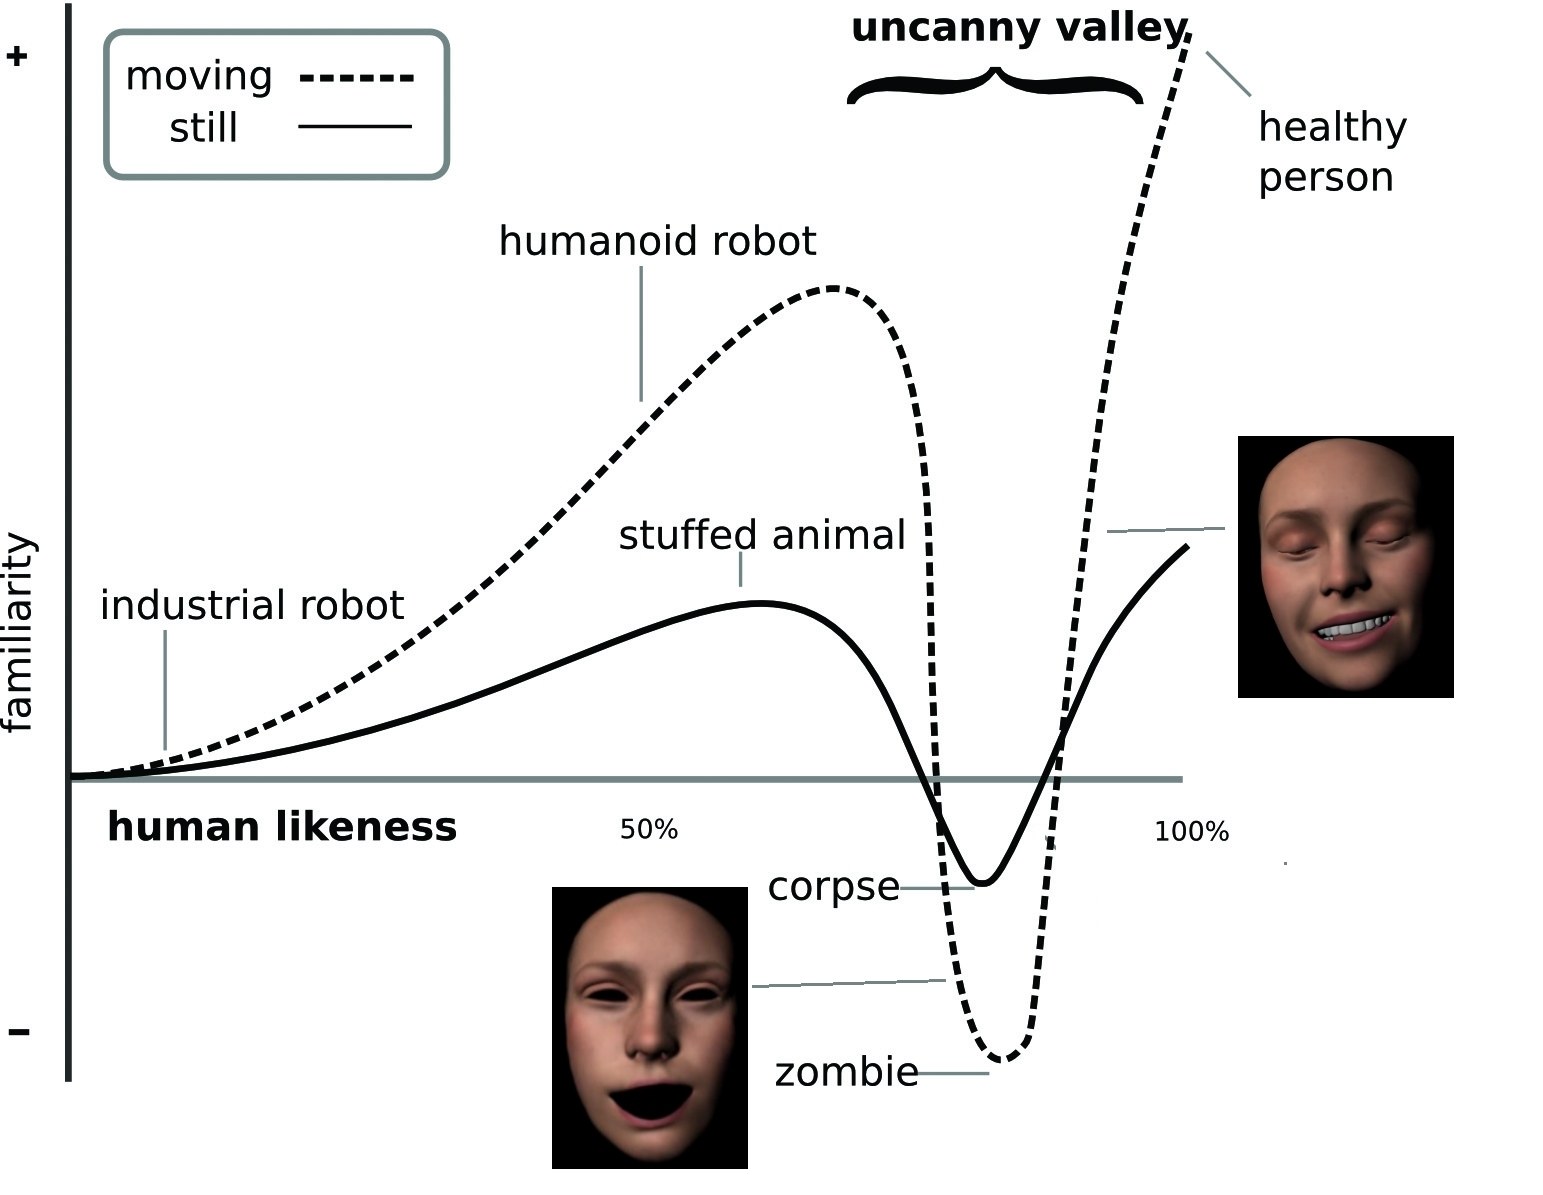
\includegraphics[width=0.8\textwidth]{img/UV}
	\caption{Our animations in the context of the uncanny valley.}
	\label{fig:UV}
\end{figure}

Despite our animation being somewhere in the uncanny valley, we believe the outcome of this project has actually been quite impressive. Not only is the final animation surprisingly life-like and true to the actor's original performance when just based upon the movements of a number of sparse markers on the face, but we have shown that it is possible to achieve a good quality performance-driven facial animation just by using standard and in-expensive off-the-shelf consumer-level tools. We don't use complicated synchronised cameras and lighting rigs - we use standard consumer level DSLR cameras, we use markers hand-drawn on the face with a make-up pencil, and we make use of a free and readily available 3D blendshape rig. This shows the power of the blendshape animation technique and what can be achieved.

In terms of rendering, doubling the resolution of the texture for the Emily model provided an improvement in the realism in the final animation.
This enhancement is mostly noticeable on close up views, where in medium distance or further shots it provides marginal to unnoticeable gains in quality.
It should be noted that, even though the texture super-resolution technique is quite computationally expensive to generate, once it is done, it will benefit every frame of the animation without any further costs.


\section{Future Work}

There are number of ways we could possibly improve the resulting facial animation, starting with the way we obtain the motion capture data. Using properly synchronised cameras at higher frame-rates (around 200fps) would significantly aid with tracking and reduce reconstruction errors. Tracking needs to be improved by incorporating a local probabilistic model, as well as global tracking, to cope with occlusions and be more robust to non-rigid deformation. We were also never able to fully remove the rigid head motion with Procrustes alignment, which then affects the resulting blendshapes since this rigid movement gets incorporated into the displacements from the neutral expression. So tracking rigid markers on the head would be helpful, or exploring alternative methods to remove this such as using non-rigid ICP or fitting some underlying model of the head which is aligned on every frame. Alternatively, we could make use of the Vicon Cara system \cite{Cara}, where the actor wears head-mounted cameras, although there will always be some minor head movement even with this. Other things we would like to investigate would be ways in which to track the movement of the eye-lids as they open, close, and squint etc. Additionally, tracking points on inside of the lips would help in the accuracy of the blendshape solve of certain expressions involving the mouth, which is one of the areas our current system struggles with.

There are a number of different techniques that could be used to construct blendshapes in the actor's domain. Deng \textit{et al}. proposed designing the blendshapes by hand~\cite{Deng:2006}. In particular, the authors choose a number of characteristic frames in the motion capture sequence, and manually design a set of shapes that perceptually match the expressions observed in these frames. They then form correspondences between the PCA coefficients of motion capture frames and the weights of the blendshapes. Finally, Radial Basis Functions are used to map the new frames in the sequence onto the three-dimensional model to produce the animation. Another option would be to use a muscle actuation basis, proposed by Choe and Ko~\cite{Choe:2005}. The design of a muscle actuation basis is based on the human facial anatomy, and is driven by the actuation of different facial muscles. Our main reservation about these approach is the extensive manual effort required to design the set of initial correspondences between the chosen frames and the three-dimensional mesh.

The accuracy of the model may be improved by taking extra care when matching the sparse points on Emily and the actor. One possible approach involves drawing a number of stable points on Emily and the actor and finding the mapping that transforms sparse Emily points to the actor's domain. Then a large number of additional points are drawn on Emily, and the same transformation is used to transform these points to the actor's domain. These points are then used to identify the ideal location of the markers on the actor's face. Moreover, a 3D printed mask may be used to ensure high accuracy when placing the markers. % THIS PARAGRAPH DOESN'T SOUND RIGHT. I FORGOT WHAT I WAS TRYING TO DAY.

The main weakness of the current method is the amount of manual work that needs to be done before the animation takes its final shape. 
% We could track eyelids and add blinks automatically.
% Including wrinkles.

The realism of the final animation could also be enhanced by applying more complex skin rendering techniques.
In this line, we could add layered materials which model subsurface scattering in the skin \cite{Weyrich2006}.
A further extension would be to include haemoglobin related phenomena, as proposed by~\cite{Donner2008, Jimenez2010}.
Adding bump maps or normals maps also increases the quality of the final result, however a light stage  is needed to acquire such data with enough resolution~\cite{Graham2013}.